\normalfalse \difficiletrue \tdifficilefalse
\correctionfalse

%\UPSTIidClasse{11} % 11 sup, 12 spé
%\newcommand{\UPSTIidClasse}{12}

\exer{Calcul vectoriel \label{CIN:01:1024}}
\setcounter{question}{0}
\marginnote{\xpComp{CIN}{01}}%\UPSTIcompetence{B2-13}
\index{Compétence B2-13-PTSI}
\index{Compétence CIN-01}

\ifcorrection
\else
\marginnote{\textbf{Pas de corrigé pour cet exercice.}}
\fi

\ifprof
\begin{figure}[H]
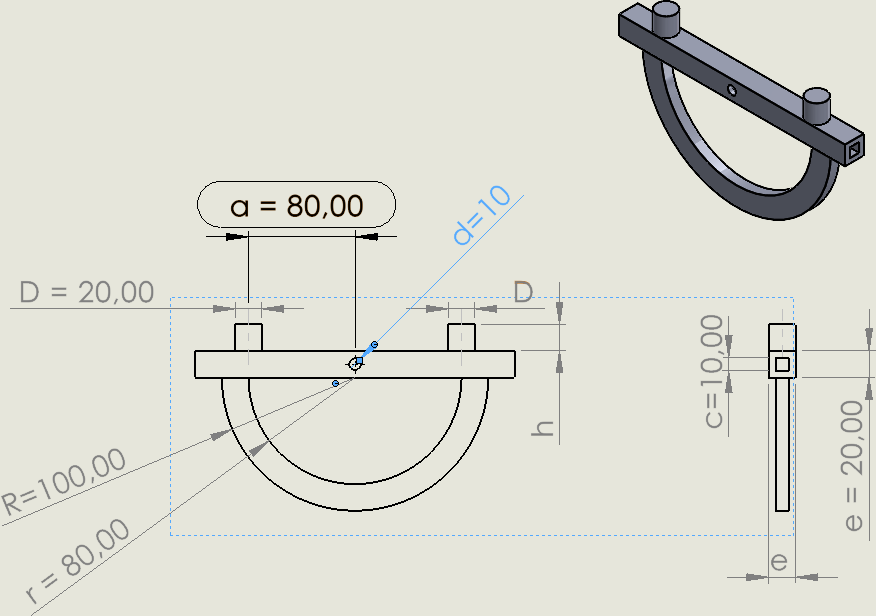
\includegraphics[width=\linewidth]{1024_01}
\end{figure}
\else
Soit les figures de changement de base suivantes. 
\begin{figure}[H]
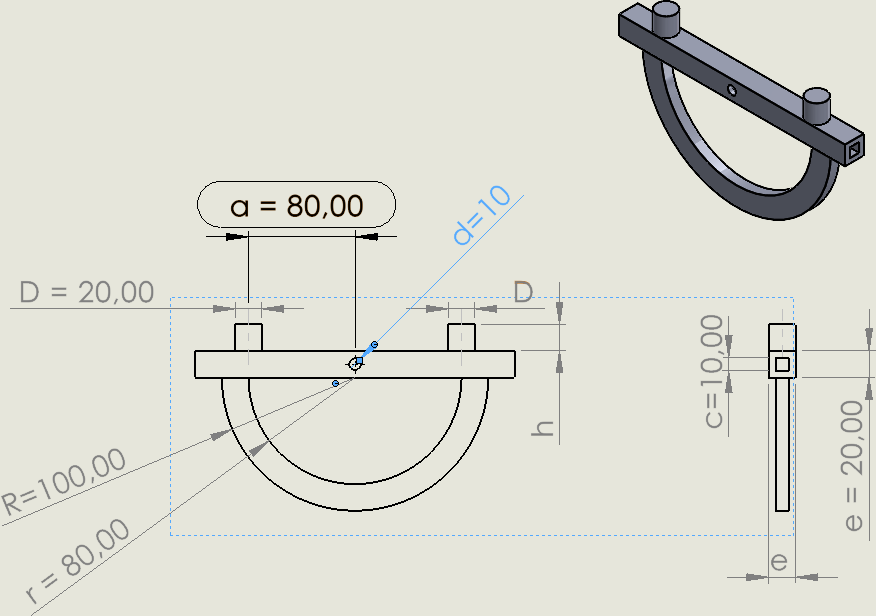
\includegraphics[width=\linewidth]{1024_01}
\end{figure}
\fi




%from itertools import combinations
%import random as rd
%vecteurs = ["\\vect{x}","\\vect{y}","\\vect{z}",
%            "\\vect{u}","\\vect{v}","\\vect{w}",
%            "\\vx{1}","\\vy{1}","\\vz{1}"]
%rd.shuffle(vecteurs)
%
%for y in combinations(vecteurs, 3):
%    print("\item : $\left("+y[0]+"\wedge"+y[1]+"\\right)\cdot"+y[2]+"$;")


    
\question{Calculer les produits vectoriels suivants :}

\ifprof~\\
\begin{enumerate}
\item : $\vect{u}\wedge\vect{w} = \vect{z_1}$
\item : $\vect{u}\wedge\vect{y} = -\sin\psi \vect{z}$
\item : $\vect{u}\wedge\vect{x} = -\sin\psi \vect{z}$
\item : $\vect{u}\wedge\vx{1} = \sin\varphi \vect{z_1}$
\item : $\vect{u}\wedge\vect{z} = -\vect{v}$
\item : $\vect{u}\wedge\vy{1} =  \cos\varphi \vect{z_1}$
\item : $\vect{u}\wedge\vz{1} = -\vect{w}$
\item : $\vect{u}\wedge\vect{v} = \vect{z_1}$
\item : $\vect{w}\wedge\vect{y} = \left( \cos\theta \vect{v}+\sin\theta \vect{z}\right)\wedge\vect{y} = -\cos\theta  \sin \psi \vect{z}-\sin\theta \vect{x}$.
\item : $\vect{w}\wedge\vect{x} =\left( \cos\theta \vect{v}+\sin\theta \vect{z}\right)\wedge\vect{x} = -\cos\theta\cos\psi \vect{z}+\sin\theta \vect{y}$
\item : $\vect{w}\wedge\vx{1} = $
\item : $\vect{w}\wedge\vect{z} = $
\item : $\vect{w}\wedge\vy{1} = $
\item : $\vect{w}\wedge\vz{1} = $
\item : $\vect{w}\wedge\vect{v} = $
\item : $\vect{y}\wedge\vect{x} = $
\item : $\vect{y}\wedge\vx{1} = $
\item : $\vect{y}\wedge\vect{z} = $
\item : $\vect{y}\wedge\vy{1} = $
\item : $\vect{y}\wedge\vz{1} = $
\item : $\vect{y}\wedge\vect{v} = $
\item : $\vect{x}\wedge\vx{1} = $
\item : $\vect{x}\wedge\vect{z} = $
\item : $\vect{x}\wedge\vy{1} = $
\item : $\vect{x}\wedge\vz{1} = $
\item : $\vect{x}\wedge\vect{v} = $
\item : $\vx{1}\wedge\vect{z}$
\item : $\vx{1}\wedge\vy{1} = $
\item : $\vx{1}\wedge\vz{1} = $
\item : $\vx{1}\wedge\vect{v} = $
\item : $\vect{z}\wedge\vy{1} = $
\item : $\vect{z}\wedge\vz{1} = $
\item : $\vect{z}\wedge\vect{v} = $
\item : $\vy{1}\wedge\vz{1} = $
\item : $\vy{1}\wedge\vect{v} = $
\item : $\vz{1}\wedge\vect{v} = $
\end{enumerate}
\else
\begin{multicols}{2}
\begin{enumerate}
\item : $\vect{u}\wedge\vect{w} = $
\item : $\vect{u}\wedge\vect{y} = $
\item : $\vect{u}\wedge\vect{x} = $
\item : $\vect{u}\wedge\vx{1} = $
\item : $\vect{u}\wedge\vect{z} = $
\item : $\vect{u}\wedge\vy{1} = $
\item : $\vect{u}\wedge\vz{1} = $
\item : $\vect{u}\wedge\vect{v} = $
\item : $\vect{w}\wedge\vect{y} = $
\item : $\vect{w}\wedge\vect{x} =  $
\item : $\vect{w}\wedge\vx{1} =  $
\item : $\vect{w}\wedge\vect{z} = $
\item : $\vect{w}\wedge\vy{1} = $
\item : $\vect{w}\wedge\vz{1} = $
\item : $\vect{w}\wedge\vect{v} = $
\item : $\vect{y}\wedge\vect{x} = $
\item : $\vect{y}\wedge\vx{1} = $
\item : $\vect{y}\wedge\vect{z} = $
\item : $\vect{y}\wedge\vy{1} = $
\item : $\vect{y}\wedge\vz{1} = $
\item : $\vect{y}\wedge\vect{v} = $
\item : $\vect{x}\wedge\vx{1} = $
\item : $\vect{x}\wedge\vect{z} = $
\item : $\vect{x}\wedge\vy{1} = $
\item : $\vect{x}\wedge\vz{1} = $
\item : $\vect{x}\wedge\vect{v} = $
\item : $\vx{1}\wedge\vect{z} = $
\item : $\vx{1}\wedge\vy{1} = $
\item : $\vx{1}\wedge\vz{1} = $
\item : $\vx{1}\wedge\vect{v} = $
\item : $\vect{z}\wedge\vy{1} = $
\item : $\vect{z}\wedge\vz{1} = $
\item : $\vect{z}\wedge\vect{v} = $
\item : $\vy{1}\wedge\vz{1} = $
\item : $\vy{1}\wedge\vect{v} = $
\item : $\vz{1}\wedge\vect{v} = $
\end{enumerate}
\end{multicols}
\fi


\question{Calculer les produits mixtes suivants :}
\begin{multicols}{2}
\begin{enumerate}
\item : $\left(\vect{z}\wedge\vz{1}\right)\cdot\vx{1} = $
\item : $\left(\vect{z}\wedge\vz{1}\right)\cdot\vect{u} = $
\item : $\left(\vect{z}\wedge\vz{1}\right)\cdot\vect{v} = $
\item : $\left(\vect{z}\wedge\vz{1}\right)\cdot\vy{1} = $
\item : $\left(\vect{z}\wedge\vz{1}\right)\cdot\vect{x} = $
\item : $\left(\vect{z}\wedge\vz{1}\right)\cdot\vect{y} = $
\item : $\left(\vect{z}\wedge\vz{1}\right)\cdot\vect{w} = $
\item : $\left(\vect{z}\wedge\vx{1}\right)\cdot\vect{u} = $
\item : $\left(\vect{z}\wedge\vx{1}\right)\cdot\vect{v} = $
\item : $\left(\vect{z}\wedge\vx{1}\right)\cdot\vy{1} = $
\item : $\left(\vect{z}\wedge\vx{1}\right)\cdot\vect{x} = $
\item : $\left(\vect{z}\wedge\vx{1}\right)\cdot\vect{y} = $
\item : $\left(\vect{z}\wedge\vx{1}\right)\cdot\vect{w} = $
\item : $\left(\vect{z}\wedge\vect{u}\right)\cdot\vect{v} = $
\item : $\left(\vect{z}\wedge\vect{u}\right)\cdot\vy{1} = $
\item : $\left(\vect{z}\wedge\vect{u}\right)\cdot\vect{x} = $
\item : $\left(\vect{z}\wedge\vect{u}\right)\cdot\vect{y} = $
\item : $\left(\vect{z}\wedge\vect{u}\right)\cdot\vect{w} = $
\item : $\left(\vect{z}\wedge\vect{v}\right)\cdot\vy{1} = $
\item : $\left(\vect{z}\wedge\vect{v}\right)\cdot\vect{x} = $
\item : $\left(\vect{z}\wedge\vect{v}\right)\cdot\vect{y} = $
\item : $\left(\vect{z}\wedge\vect{v}\right)\cdot\vect{w} = $
\item : $\left(\vect{z}\wedge\vy{1}\right)\cdot\vect{x} = $
\item : $\left(\vect{z}\wedge\vy{1}\right)\cdot\vect{y} = $
\item : $\left(\vect{z}\wedge\vy{1}\right)\cdot\vect{w} = $
\item : $\left(\vect{z}\wedge\vect{x}\right)\cdot\vect{y} = $
\item : $\left(\vect{z}\wedge\vect{x}\right)\cdot\vect{w} = $
\item : $\left(\vect{z}\wedge\vect{y}\right)\cdot\vect{w} = $
\item : $\left(\vz{1}\wedge\vx{1}\right)\cdot\vect{u} = $
\item : $\left(\vz{1}\wedge\vx{1}\right)\cdot\vect{v} = $
\item : $\left(\vz{1}\wedge\vx{1}\right)\cdot\vy{1} = $
\item : $\left(\vz{1}\wedge\vx{1}\right)\cdot\vect{x} = $
%\item : $\left(\vz{1}\wedge\vx{1}\right)\cdot\vect{y} = $
%\item : $\left(\vz{1}\wedge\vx{1}\right)\cdot\vect{w} = $
%\item : $\left(\vz{1}\wedge\vect{u}\right)\cdot\vect{v} = $
%\item : $\left(\vz{1}\wedge\vect{u}\right)\cdot\vy{1} = $
%\item : $\left(\vz{1}\wedge\vect{u}\right)\cdot\vect{x} = $
%\item : $\left(\vz{1}\wedge\vect{u}\right)\cdot\vect{y} = $
%\item : $\left(\vz{1}\wedge\vect{u}\right)\cdot\vect{w} = $
%\item : $\left(\vz{1}\wedge\vect{v}\right)\cdot\vy{1} = $
%\item : $\left(\vz{1}\wedge\vect{v}\right)\cdot\vect{x} = $
%\item : $\left(\vz{1}\wedge\vect{v}\right)\cdot\vect{y} = $
%\item : $\left(\vz{1}\wedge\vect{v}\right)\cdot\vect{w} = $
%\item : $\left(\vz{1}\wedge\vy{1}\right)\cdot\vect{x} = $
%\item : $\left(\vz{1}\wedge\vy{1}\right)\cdot\vect{y} = $
%\item : $\left(\vz{1}\wedge\vy{1}\right)\cdot\vect{w} = $
%\item : $\left(\vz{1}\wedge\vect{x}\right)\cdot\vect{y} = $
%\item : $\left(\vz{1}\wedge\vect{x}\right)\cdot\vect{w} = $
%\item : $\left(\vz{1}\wedge\vect{y}\right)\cdot\vect{w} = $
%\item : $\left(\vx{1}\wedge\vect{u}\right)\cdot\vect{v} = $
%\item : $\left(\vx{1}\wedge\vect{u}\right)\cdot\vy{1} = $
%\item : $\left(\vx{1}\wedge\vect{u}\right)\cdot\vect{x} = $
%\item : $\left(\vx{1}\wedge\vect{u}\right)\cdot\vect{y} = $
%\item : $\left(\vx{1}\wedge\vect{u}\right)\cdot\vect{w} = $
%\item : $\left(\vx{1}\wedge\vect{v}\right)\cdot\vy{1} = $
%\item : $\left(\vx{1}\wedge\vect{v}\right)\cdot\vect{x} = $
%\item : $\left(\vx{1}\wedge\vect{v}\right)\cdot\vect{y} = $
%\item : $\left(\vx{1}\wedge\vect{v}\right)\cdot\vect{w} = $
%\item : $\left(\vx{1}\wedge\vy{1}\right)\cdot\vect{x} = $
%\item : $\left(\vx{1}\wedge\vy{1}\right)\cdot\vect{y} = $
%\item : $\left(\vx{1}\wedge\vy{1}\right)\cdot\vect{w} = $
%\item : $\left(\vx{1}\wedge\vect{x}\right)\cdot\vect{y} = $
%\item : $\left(\vx{1}\wedge\vect{x}\right)\cdot\vect{w} = $
%\item : $\left(\vx{1}\wedge\vect{y}\right)\cdot\vect{w} = $
%\item : $\left(\vect{u}\wedge\vect{v}\right)\cdot\vy{1} = $
%\item : $\left(\vect{u}\wedge\vect{v}\right)\cdot\vect{x} = $
%\item : $\left(\vect{u}\wedge\vect{v}\right)\cdot\vect{y} = $
%\item : $\left(\vect{u}\wedge\vect{v}\right)\cdot\vect{w} = $
%\item : $\left(\vect{u}\wedge\vy{1}\right)\cdot\vect{x} = $
%\item : $\left(\vect{u}\wedge\vy{1}\right)\cdot\vect{y} = $
%\item : $\left(\vect{u}\wedge\vy{1}\right)\cdot\vect{w} = $
%\item : $\left(\vect{u}\wedge\vect{x}\right)\cdot\vect{y} = $
%\item : $\left(\vect{u}\wedge\vect{x}\right)\cdot\vect{w} = $
%\item : $\left(\vect{u}\wedge\vect{y}\right)\cdot\vect{w} = $
%\item : $\left(\vect{v}\wedge\vy{1}\right)\cdot\vect{x} = $
%\item : $\left(\vect{v}\wedge\vy{1}\right)\cdot\vect{y} = $
%\item : $\left(\vect{v}\wedge\vy{1}\right)\cdot\vect{w} = $
%\item : $\left(\vect{v}\wedge\vect{x}\right)\cdot\vect{y} = $
%\item : $\left(\vect{v}\wedge\vect{x}\right)\cdot\vect{w} = $
%\item : $\left(\vect{v}\wedge\vect{y}\right)\cdot\vect{w} = $
%\item : $\left(\vy{1}\wedge\vect{x}\right)\cdot\vect{y} = $
%\item : $\left(\vy{1}\wedge\vect{x}\right)\cdot\vect{w} = $
%\item : $\left(\vy{1}\wedge\vect{y}\right)\cdot\vect{w} = $
%\item : $\left(\vect{x}\wedge\vect{y}\right)\cdot\vect{w} = $
\end{enumerate}
\end{multicols}
\ifprof~\\
\else
\fi



\ifprof
\else

\footnotesize

\normalsize


\marginnote{Corrigé voir \ref{CIN:01:B2:13:PTSI:46}.}

\fi